\documentclass[12pt]{article}
\usepackage[letterpaper]{geometry}
%\textwidth = 345.0pt
%\hoffset = -3cm
\usepackage[utf8]{inputenc}
\usepackage[spanish,es-tabla]{babel}
\usepackage[autostyle,spanish=mexican]{csquotes}
\usepackage{amsmath}
\usepackage{nccmath}
\usepackage{amsthm}
\usepackage{amssymb}
\usepackage{graphicx}
\usepackage{comment}
\usepackage{siunitx}
\usepackage{physics}
\usepackage{color}
\usepackage{float}
\usepackage{multicol}
%\usepackage{milista}
\usepackage{enumitem}
\usepackage{anyfontsize}
\usepackage{anysize}
\marginsize{1cm}{1cm}{1cm}{1cm}
\usepackage{enumitem}
\usepackage{capt-of}
\usepackage{bm}
\usepackage{relsize}
\newlist{milista}{enumerate}{2}
\setlist[milista,1]{label=\arabic*)}
\setlist[milista,2]{label=\arabic{milistai}.\arabic*)}
\spanishdecimal{.}
\renewcommand{\baselinestretch}{1.5}
\author{ }
\title{Problemas para la Tarea - Examen del Tema 4 \\ \large{Matemáticas Avanzadas de la Física} \vspace{-1.5\baselineskip}}
\date{ }
\begin{document}
\vspace{-4cm}
%\renewcommand\theenumii{\arabic{theenumii.enumii}}
\renewcommand\labelenumii{\theenumi.{\arabic{enumii})}}
\maketitle
\fontsize{14}{14}\selectfont
\begin{enumerate}
\item En una distribución tipo Maxwell la fracción de partículas moviéndose con velocidad $v$ y $v +\dd{v}$ es
\begin{align*}
\dfrac{\dd{N}}{N} = 4 \, \pi \left( \dfrac{m}{2 \, \pi \, k \, T} \right)^{3/2} \: \exp \left( \dfrac{-m \, v^{2}}{k \, T} \right) \: v^{2} \dd{v}
\end{align*}
donde $N$ es el número total de partículas. El promedio o valor esperado de $v^{n}$ se define como $\displaystyle \expval{v^{n}} = N^{-1} \int v^{n} \dd{N}$. Demostrar que
\begin{align*}
\expval{v^{n}} = \left( \dfrac{2 \, k \, T}{m} \right)^{n/2} \dfrac{\left( \dfrac{n + 1}{2} \right) !} { \left( \dfrac{1}{2} \right) !}
\end{align*}
\item Demostrar que
\begin{align*}
\int_{0}^{\infty} e^{-x^{4}} \dd{x} = \left( \dfrac{1}{4} \right) !
\end{align*}
\item Comprueba las siguientes identidades de la función Beta:
\begin{enumerate}
\setlength{\itemsep}{15pt}
%\item $B(a, b) = B(a + 1, b) + B(a, b + 1)$
%\item $B(a, b) = \dfrac{a + b}{b} B(a, b + 1)$ 
\item $B(a, b) = \dfrac{b - 1}{a} \, B (a + 1, b - 1)$
\item $B(a, b) \, B(a + b, c) = B(b, c) \, B(a, b + c)$
\end{enumerate}
\item Demostrar que
\begin{align*}
\int_{-1}^{1} (1-x^{2})^{1/2} \: x^{2 \, n} \dd{x} =  
\begin{cases}
\pi/2 & n = 0 \\[1em]
\pi \dfrac{(2 \, n - 1)!!}{(2 \, n + 2)!!} & n = 1,2,3,\ldots  \end{cases}
\end{align*} 
\item Demuestra que 
\begin{align*}
\Gamma \left( \dfrac{1}{2} - n \right) \: \Gamma \left( \dfrac{1}{2} + n \right) = (-1)^{n} \: \pi
\end{align*}
\newpage
\item Expresa las siguientes integrales como funciones Beta, para luego dejarlas en términos de funciones Gamma, y evalúa cada de ellas.
\begin{enumerate}
\item $\displaystyle \int_{0}^{1} \dfrac{x^{4}}{\sqrt{1 -x^{2}}} \dd{x}$
\item $\displaystyle \int_{0}^{1} x^{2} \, (1 - x^{2})^{3/2} \dd{x}$
\end{enumerate} 
\item En la siguiente figura (\ref{fig:figura_01}) se aprecia la curva determinada por la expresión
\begin{align*}
x^{b/c} + y^{b/c} = a^{b/c}
\end{align*}
donde: $a$ es una constante positiva, $b$ es un entero par positivo y $c$ es un entero impar positivo. Calcula el área dentro de la curva cuando el exponente $b/c$ es $2/3$, en términos de la función Gamma.
\begin{figure}[!ht]
    \centering
    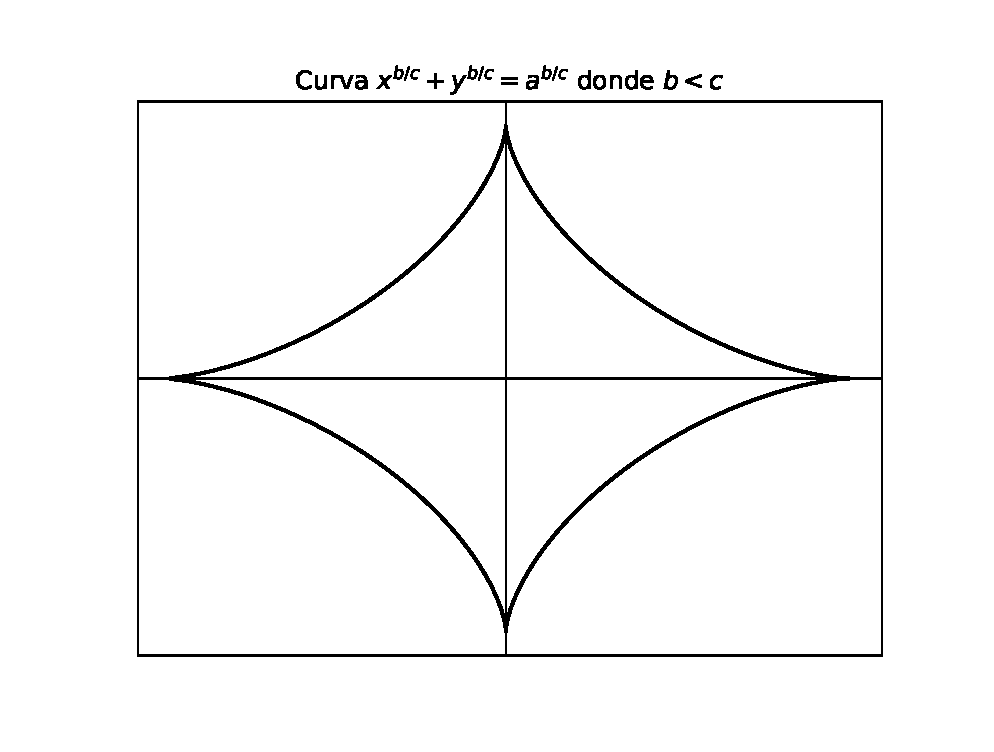
\includegraphics[scale=0.8]{Imagenes/plot_curva_estrella_01.eps}
    \caption{Estrella con cuatro picos cóncavos.}
    \label{fig:figura_01}
\end{figure}
\item Un carro está estacionado con la puerta abierta en ángulo recto $(\theta = \ang{90})$, cuando de repente se enciende el carro y acelera de manera constante $a = \SI{1}{\kilo\meter\hour\per\second}$. La ED para $\theta(t)$ es
\begin{align*}
\theta (t) =  \ddot{\theta} - A \, \sin \theta
\end{align*}
donde $A = 3a/2w$, para una puerta estándar de ancho $w$. Si $w = \SI{1.2}{\meter}$, calcula cuánto tiempo tarda en cerrarse la puerta.
%\newpage
\item Se muestra en la figura (\ref{fig:figura_02}) parte de una cicloide cuyas ecuaciones paramétricas son
\begin{align*}
x = a (\theta + \sin \theta) \hspace{1.5cm} y = a (1 - \cos \theta)
\end{align*}
\begin{figure}[H]
    \centering
    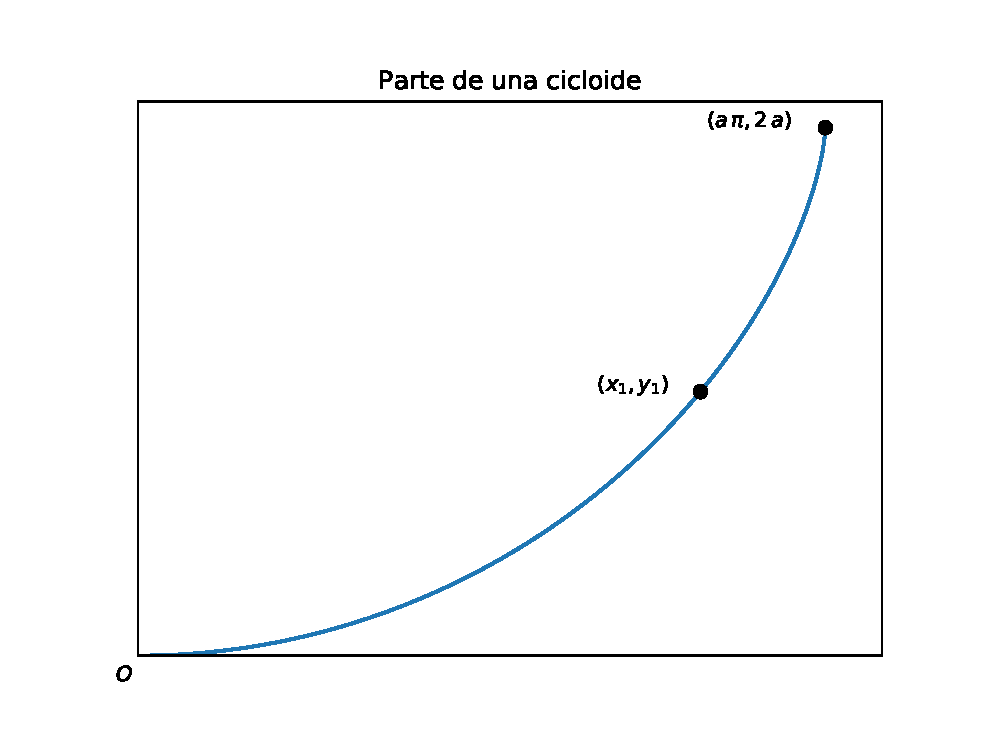
\includegraphics[scale=0.7]{Imagenes/plot_cicloide.eps}
    \caption{Una partícula deslizándose sobre una cicloide.}
    \label{fig:figura_02}
\end{figure}
Demuestra que el tiempo que tarda una partícula para deslizarse sin fricción a lo largo de la curva desde el punto $(x_{1}, y_{1})$ hasta el origen, está dado por
\begin{align*}
t = \sqrt{\dfrac{a}{g}} \int_{0}^{y_{1}} \dfrac{\dd{y}}{\sqrt{y (y_{1}- y)}}
\end{align*}
Sugerencia: Demuestra que la longitud del elemento de arco es $\dd{s} = \sqrt{2a/y} \dd{y}$. Evalúa la integral para demostrar que el tiempo es independiente de la posición inicial $y_{1}$.
\item Partiendo del siguiente resultado
\begin{align*}
\Gamma \left( \dfrac{1}{2} \right) = \int_{0}^{\infty} \dfrac{e^{-t} \dd{t}}{\sqrt{t}}
\end{align*}
y con la transformación $y^{2} = t$ o $x^{2}=t$. Demuestra que
\begin{align*}
\left[ \Gamma \left( \dfrac{1}{2} \right) \right]^{2} = 4 \,  \int_{0}^{\infty} \, \int_{0}^{\infty} \exp[-(x^{2} + y^{2})] \dd{x} \dd{y}
\end{align*}
Una vez demostrado, ahora usa la integral doble sobre el primer cuadrante y que cuando se evalúa utilizando coordenadas polares $(r, \theta)$, se obtiene
\begin{align*}
\Gamma \left( \dfrac{1}{2} \right) = \sqrt{\pi}
\end{align*}
\end{enumerate}
\end{document}